%% -*- coding: utf-8; -*-

% Use 'digital' option to enable back references. This option is recommended for digital pdf version
%\documentclass[phd,american,digital]{thesispuc}%english thesis
%\documentclass[mscr,american]{thesispuc}%english dissertation
%\documentclass[phd,brazilian]{thesispuc}%tese em portugês
\documentclass[msc,brazilian]{thesispuc}%disseretação em portuguŝ


%%%
%%% Additional Packages
%%%
\usepackage{tabularx}
\usepackage{multirow}
\usepackage{multicol}
\usepackage{colortbl}
\usepackage[%
    dvipsnames,
    svgnames,
    x11names,
    fixpdftex,
    table
]{xcolor}
\usepackage{numprint}
\usepackage{textcomp}
\usepackage{booktabs}
\usepackage{amsmath}
\usepackage{enumitem}
\usepackage{amssymb}
% ABNT reference style package. The current style is the alphabetical order, if you need
% change to citation order, change in the line above 'alf' to 'num', also at the end replace
% bibliographystyle with the commented version.
\usepackage[num]{abntex2cite}
%\usepackage{tikz}
%\usepackage[linesnumbered, ruled, vlined]{algorithm2e}
%\usepackage{pgfplots,pgfplotstable} 
%\usepackage{array}

%% numprint 
\npthousandsep{.}
\npdecimalsign{,}

%% ThesisPUC option
%\tablesmode{fig} %% [nada, fig, tab ou figtab]
%\algoritmsmode{none} %% [none ou use] %% Default is [use]
%\codesmode{none} %% [none ou use] %% Default is [use]
%\abreviationsmode{none} %% [none ou use] %% Default is [use]
\tablesmode{none}
\algorithmsmode{none}
\codesmode{none}
\abreviationsmode{none}

% \makeatletter  \renewcommand\@biblabel[1]{#1}  \makeatother

%%%
%%% Counters
%%%

%% uncomment and change for other depth values
\setcounter{tocdepth}{1}
%\setcounter{lofdepth}{3}
%\setcounter{lotdepth}{3}
%\setcounter{secnumdepth}{3}

%%%
%%% Misc.
%%%

\usecolour{true}
%% \graphicspath{ {./figuras/} }
%% https://www.overleaf.com/learn/latex/Inserting_Images
\citebrackets[]


%%%
%%% Titulos
%%%

\autor{Daniel Schreiber Guimarães}
\autorR{Guimarães, Daniel Schreiber}

\advisor{Marcos Vianna Villas}{Prof.}
\advisorR{Villas, Marcos Vianna}
% If the advisor's department is different from author's department, uncomment the next line and type the correct name and acronym of advisor's institution.
%\advisorInst{institution name}{acronym}

%\coadvisor{Otávio da Fonseca Martins Gomes}{Dr.}
%\coadvisorR{da Fonseca Martins Gomes, Otávio}
%\coadvisorInst{Centro de Tecnologia Mineral}{CETEM/MCTI}

\title{Sistema de recomendação de disciplinas para matrícula de um aluno da PUC-Rio}

%%\subtitulo{Aqui vai o subtitulo caso precise}

\day{02}
\month{Maio}
\year{2023}

\city{Rio de Janeiro}
\CDD{004} 
\department{Informática}
\program{Engenharia da Computação}
\school{Engenharia da Computação}
\university{Pontifícia Universidade Católica do Rio de Janeiro}
\uni{PUC-Rio}


%%%
%%% Jury
%%%

\jury{%
  \jurymember{Alberto Barbosa Raposo}{Prof.}
    {Departamento de Informática}{PUC-Rio}
  \jurymember{Waldemar Celes Filho}{Prof.}
    {Departamento de Informática}{PUC-Rio}
}


%%%
%%% Personal Resume
%%%

\resume{%
% If it fit in one line use this command:
\makebox[\textwidth][s]{Graduando em Engenharia da Computação na PUC - Rio}%
% If not just type your resume without any special command 
}

%%%
%%% Acknowledgment (REMINDER TO SCHOLARSHIP STUDENTS. Do not forget to thank the agencies that supported your work.)
%%% REMOVIDO POR DANIEL
%%%
% \acknowledgment{%
% \noindent To my adviser Professor Marcelo Gattass for the stimulus and partnership
% to carry out this work.
% \bigskip

% \noindent To CNPq and PUC-Rio, for the aids granted, without which this work does not
% could have been accomplished.
% \bigskip
% }


%%%
%%% Catalog prekeywords
%%%

\catalogprekeywords{%
  \catalogprekey{Informática}%
}

%%%
%%% Keywords - Don't use % at the end of /key dfinition
%%%

\keywords{%
  \key{Recomendação}
  \key{Disciplinas}
  % \key{Imagens de Exames médicos}
  % \key{Vizinhança adaptativa}
}

\keywordsuk{%
  \key{Recommendation}
  \key{Courses}
}


%%%
%%% Abstract
%%%

\abstract{%
Esse resumo ainda será preenchido.
}

\abstractuk{%
This abstract will be filled.
}


%%%
%%% Dedication
%%%

\dedication{%
  Para os meus pais, por\\todo o seu suporte e encorajamento.
}

%%%
%%% Epigraph (removido manualmente pelo thesispuc.cls)
%%%

% \epigraph{%
% }
% \epigraphauthor{Wassily Kandinsky}
% \epigraphbook{Regards sur le passé}


\begin{document}
  % -*- coding: utf-8; -*-

\chapter{Introdução}

A cada semestre, um aluno que está fazendo graduação no Departamento de Informática da PUC-Rio precisa fazer a sua matrícula em disciplinas oferecidas pela universidade para os próximos seis meses. Apesar de algumas restrições como pré-requisitos de disciplinas, o aluno tem ampla liberdade de escolher as disciplinas que melhor se encaixam na sua grade horária. Essa liberdade é uma vantagem devido à disponibilização de uma grade horária flexível para o aluno, porém precisa de um maior esforço de pesquisa e organização deste aluno para que a sua matrícula no próximo período seja feita de forma eficaz segundo critérios do próprio aluno. 

A motivação desse projeto é o estudo, planejamento e desenvolvimento de um sistema de recomendação de disciplinas para o próximo período que auxilie o aluno em sua matrícula ao sugerir interativamente disciplinas com base em dados fornecidos pela universidade e por avaliações informadas por alunos.
  % -*- coding: utf-8; -*-

\chapter{Situa{\c c}\~ao Atual}
\label{cha:Situa{\c c}\~ao Atual}

\section{Serviços disponibilizados}

O microhorario\footnote{https://www.puc-rio.br/microhorario} é um serviço disponibilizado pela universidade para consultar informações das disciplinas do semestre atual. Este possui uma interface simples que pode ser visualizada na figura \ref{fig:microhorario}. Essa interface permite filtrar disciplinas por seus atributos como nome, código, professor e departamento. Porém, essa interface não é personalizada com relação ao aluno, ou seja, não exibe as disciplinas que o aluno em específico ainda não cursou ou que o aluno não pode cursar devido à pré-requisitos.

\begin{figure}[h]
    \begin{center}
    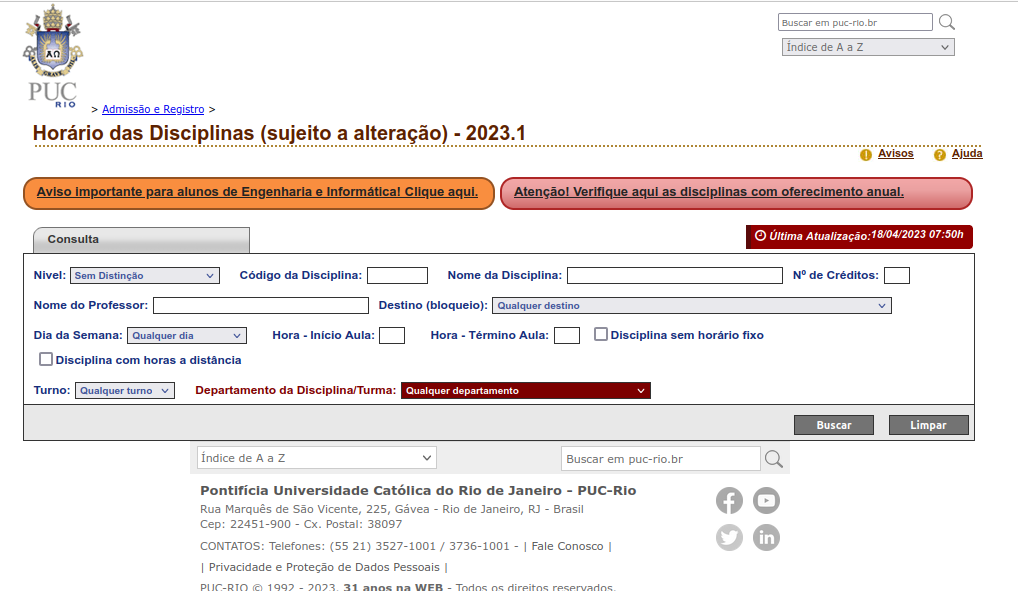
\includegraphics[width=300pt]{figuras/microhorario}
    \caption{Interface do \textit{microhorario}}
    \label{fig:microhorario}
    \end{center}
\end{figure}

Para consultar a grade recomendada e os pré-requisitos, o aluno de engenharia de computação precisa acessar um documento\footnote{http://www.inf.puc-rio.br/wordpress/wp-content/uploads/2023/01/\\Grade\_Eng\_comp\_2023.pdf} presente na página do departamento ou acessar o currículo disponibilizado na página da universidade. Outros cursos disponibilização documentos semelhantes em páginas diferentes. A grade recomendada possui os nomes das disciplinas e seus pré-requisitos, mas não contém a disponibilidade do próximo período.

Além disso, as disciplinas eletivas que o departamento oferece durante o semestre são anunciadas em diferentes veículos de comunicação, como e-mail, página da coordenação do curso, ou folhetos em corredores do departamento. Não há uma distribuição centralizada das ofertas de disciplinas eletivas, portanto o aluno pode não saber aonde procurar essas ofertas, e perder boas oportunidades por desconhecer o anúncio da disciplina eletiva.

No final de cada período, a universidade oferece um serviço de avaliação de disciplinas e professores, permitindo avalia-los em várias categorias. Porém, os resultados das avaliações não são disponíveis publicamente.

\section{Processo de matrícula}

A matrícula na PUC-Rio é um processo que dura vários dias. A universidade divulga o agendamento de matrícula, em que cada aluno recebe uma data e hora para realizar sua matrícula através do portal online do aluno. As datas possíveis abrangem um período de cinco dias. Durante o período de matrícula, o microhorario atualiza periodicamente para indicar quais turmas ainda possuem vagas disponíveis, e se houve o cadastro ou cancelamento de alguma outra disciplina durante este período.

Portanto, é comum que um aluno crie formas de planejamento próprias para conseguir organizar todo o fluxo de dependências, anotar as disciplinas que estão sendo oferecidas, assim como suas turmas e professores. Esses dados precisam estar em constante atualização durante o período de matrícula, conforme as vagas vão sendo preenchidas e a disponibilização de novas turmas ou disciplinas são anunciadas. Este é um processo que maximiza a qualidade da sua grade horária, mas demanda muito esforço e tempo. 

\begin{figure}[h]
  \begin{center}
  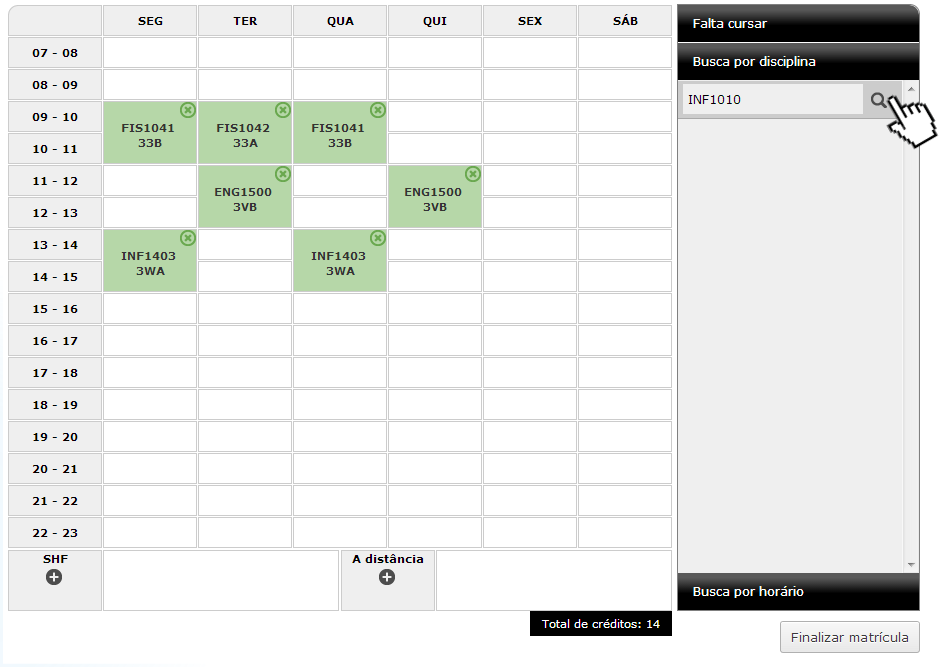
\includegraphics[width=250pt]{figuras/simulador}
  \caption{Interface do simulador}
  \label{fig:simulador}
  \end{center}
\end{figure}

A universidade disponibiliza por dois ou três dias um simulador de matrícula  antes do processo de matrícula em si. A interface do simulador é a mesma da matrícula, como pode ser observado na figura \ref{fig:simulador}, 
afim de o aluno poder simular a criação da sua grade de disciplinas para o próximo semestre. O simulador apresenta os dados das disciplinas atualizados conforme o microhorario, e os disponibiliza de três formas diferentes: buscas por disciplinas que faltam cursar no currículo do aluno, buscar por nomes de disciplinas e buscar por horários das turmas das 
disciplinas.\cite{doc-matricula}



\section{Estudos relacionados}

A escolha de disciplinas é um problema comum em universidades que possuem algum grau de flexibilidade na grade horária. Ng \& Linn\cite{crs-recs} desenvolveram um sistema de recomendação de disciplinas para a sua universidade chamado CrsRecs que utiliza análise de sentimento, pontuações de professores e disciplinas, e preferências que o aluno escolhe fornecer. A vantagem do CrsRecs é não depender de dados privados da universidade como notas e avaliação dos alunos nas disciplinas, utilizando somente informações fornecidas diretamente pelo usuário. Mas há também um esforço na decodificação das informações fornecidas, o que pode ocasionar recomendações incorretas provenientes da má interpretação do usuário.

Há estudos que utilizam históricos escolares dos alunos para gerar modelos de previsão de notas.\cite{rani-machine-learning,nguyen-learning-outcome,adak-fuzzy} Nesse caso, o objetivo do modelo é tentar prever quais disciplinas o aluno tem a maior chance de obter uma boa nota, mas não necessariamente prever quais delas mais combina com o aluno.\cite{rani-machine-learning,nguyen-learning-outcome}

A escolha de disciplinas eletivas também é uma preocupação presente nas universidades. Na PUC-Rio e em outras universidades, os currículos de graduação solicitam créditos de disciplinas eletivas, seja dentro do departamento da graduação do aluno ou não. O sistema do estudo de Adak et al.\cite{adak-fuzzy} recomenda disciplinas dentro de um departamento que parecem se relacionar com o histórico escolar do aluno, mas excluem disciplinas fora do departamento.
Já o sistema de Xu et al.\cite{xu-personalizado} recomenda uma sequência de disciplinas eletivas que maximem a sua nota e não aumentem o tempo de conclusão da graduação do aluno, levando em conta dados históricos do aluno e a disponibilidade atual das disciplinas. 
Por último, o estudo de Adak \& Ercan\cite{adak-svm} utiliza dois algoritmos de inteligência artificial de aprendizado supervisionado, support vector machine (SVM) e árvores de decisão, para recomendar eletivas que mais se combinam com o aluno, utilizando dados históricos do aluno tanto para o treinamento dos modelos de algoritmo como para a recomendação.

O comum nos estudos é a tentativa de maximizar a nota média do aluno utilizando os dados históricos de alunos da universidade para treinar modelos de inteligência artificial.\cite{rani-machine-learning,nguyen-learning-outcome,adak-fuzzy,adak-svm} Porém, o foco específico nos resultados pode ocultar oportunidades de disciplinas que o aluno poderia se interessar.

% Early smoothing methods tried to minimize... In the figure \ref{subfig:pictures/image01.png} we see...

% \subimages{A set of three subfigures:
% (a) describes the first subfigure;
% (b) describes the second subfigure;
% (c) describes the third subfigure.}{55}
% {
%  \subimage[Bamboo-pile Vertically Inserted Position]{.45}{pictures/image01.png}
%  \subimage[Bamboo-pile Normal Inserted Position]{.45}{pictures/image02.png}\\
%  \subimage[bamboo-pile Inserted 45° angle]{.45}{example-image}
% }
% \newpage
% \csubimages{A set of six subfigures in two pages.}{55}
% {
%  \subimage[Bamboo-pile Vertically Inserted Position]{.45}{pictures/image01.png}
%  \subimage[Bamboo-pile Normal Inserted Position]{.45}{pictures/image02.png}\\
%  \subimage[bamboo-pile Inserted 45° angle]{.45}{example-image}
% }
% \ssubimages{A set of six subfigures in two pages.(Continuation)}{55}
% {
%  \subimage[Bamboo-pile Vertically Inserted Position]{.45}{pictures/image01.png}
%  \subimage[Bamboo-pile Normal Inserted Position]{.45}{pictures/image02.png}\\
%  \subimage[bamboo-pile Inserted 45° angle]{.45}{example-image}
% }
  % -*- coding: utf-8; -*-
\chapter{Proposta}
\label{cha:Proposta}


O sistema proposto nesse trabalho é uma interface de planejamento de matrícula semelhante ao simulador de matrícula integrado com um algoritmo de recomendação. O sistema disponibiliza as disciplinas do próximo período conforme os dados mais atuais do microhorario. Para que haja uma personalização na recomendação das disciplinas, o sistema permitirá que o aluno carregue o histórico escolar na universidade afim de fornecer o histórico das disciplinas e seus graus para o algoritmo de recomendação.

O algoritmo de recomendação do sistema receberá as disciplinas oferecidas no próximo período e seus pré-requisitos, o modelo de grade recomendada pelo departamento e o histórico do aluno e responderá com disciplinas selecionadas pelo algoritmo. O algoritmo também poderá ser personalizado com informações de preferência do usuário que serão definidas ao longo da etapa de validação do problema.

Também será validada a proposta de armazenar o histórico fornecido pelo aluno sem os dados pessoais afim de montar uma base de dados contendo exemplos de grades de alunos e suas notas, para que o algoritmo a utilize para obter resultados mais satisfatórios para o aluno usuário do sistema.

O sistema e o algoritmo será desenvolvido especificamente para alunos do departamento de informática da PUC-Rio devido a dificuldade de abranger todas os currículos nos diferentes departamentos da universidade. Essa restrição também permite restrigir o escopo do projeto afim de tentar obter melhores resultados.

% Equation example 1:

% \begin{equation}
% \begin{split}
% \min_u \int_{x_i\in X}\int_{x_j\in X} q_{ij} u_i u_j da da + \int_{x_i\in X}||x' - x_i|| u_i da \\
% s.t. \ \ \ u\in[0,1] \ \ \land  \ \ \int_{x_i\in X}u da = a_0,
% \end{split}
% \end{equation}

% Equation exmaple 2:

% \begin{equation}
% \begin{split}
% \min_{\mathbf{u}} \alpha \mathbf{u}^T \mathbf{A}^T \mathbf{Q} \mathbf{A} \mathbf{u} +  \beta \mathbf{d}^T a' \mathbf{A} \mathbf{u} + \gamma \mathbf{u}^T \mathbf{G}^T \mathbf{G} \mathbf{u} + \delta\mathbf{f}^T a' \mathbf{A} \mathbf{u} \\
% s.t. \ \ \ \mathbf{0} \leq \mathbf{u} \leq \mathbf{1} \land \mathbf{a}^T\mathbf{u}=a_0.
% \end{split}
% \end{equation}

% Equation example 3:
% \begin{align}
% \mathbf{G}=(g_{ij}) = \left\lbrace
% \begin{array}{ll}
% \sum_{f_k\in N_f(f_i)} l_{ik} & i=j\\
% -l_{ij} & e_{ij}\in E\\
% 0 & \text{otherwise}
% \end{array}
% \right.
% \end{align}

% \lstinputlisting[label=mean,title={Mean Filter},caption={Mean Filter},language=R]{codes/mean.R}

% %% Poruguese algorithm
% %\begin{algorithm}
% %\DontPrintSemicolon
% %\Entrada{Malha e quantidade de pontos a ser amostrado}
% %\Saida{Pontos amostrados na malha}
% %\BlankLine
% %\emph{Crie um vetor de números randômicos entre $[0,1]$ com a %quantidade de pontos a ser amostrada e ordene-o}\;
% %\emph{Calcule a área total dos triângulos da malha}\;
% %\For{$i=0$ \KwTo numeroDePontos} {
% %  \emph{Navegue entre as faces acumulando a sua $\frac{area}{areaTotal}$ até achar a face com valor acumulado $\geqslant$ numerosRandomicos[i]}\;
% %  \emph{Pegue um ponto randômico dentro da face utilizando o %método de Turk e adicione no vetor do resultado}\;
% %}
% %\caption{Escolha das amostras inicias}\label{alg:sampling}
% %\end{algorithm}\DecMargin{1em}

% %% enlgish algorithm
% \begin{algorithm}
% \DontPrintSemicolon
% \KwIn{Malha e quantidade de pontos a ser amostrado}
% \KwOut{Pontos amostrados na malha}
% \BlankLine
% \emph{Crie um vetor de números randômicos entre $[0,1]$ com a quantidade de pontos a ser amostrada e ordene-o}\;
% \emph{Calcule a área total dos triângulos da malha}\;
% \For{$i=0$ \KwTo numeroDePontos} {
%   \emph{Navegue entre as faces acumulando a sua $\frac{area}{areaTotal}$ até achar a face com valor acumulado $\geqslant$ numerosRandomicos[i]}\;
%   \emph{Pegue um ponto randômico dentro da face utilizando o método de Turk e adicione no vetor do resultado}\;
% }
% \caption{Escolha das amostras inicias}\label{alg:sampling}
% \end{algorithm}\DecMargin{1em}

  % -*- coding: utf-8; -*-

\chapter{Plano de Ação}
\label{cha:Plano de Ação}

Para modelar o sistema, foi realizada uma validação do problema. Alunos do departamento de informática da universidade foram entrevistados afim de descobrir quais dificuldades enfrentam durante o processo de matrícula e quais são as suas preferências ao montar uma grade disciplinar. O objetivo era identificar quais características de uma grade disciplinar contribuem para a satisfação do aluno e adicionar as funcionalidades necessárias no sistema e no algoritmo.

Com o problema validado, então o projeto passou por uma etapa de pesquisa. 
Foram estudados diferentes algoritmos de recomendação em contextos semelhantes ao sistema a ser desenvolvido, afim de se projetar o algoritmo que mais se adequa às necessidades do problema validado. 
Nessa etapa, também foram analisadas as fontes de informações disponibilizadas pela universidade e como cada fonte pode ser integrada no sistema. 
Por exemplo, já existia uma biblioteca\footnote{Dispon\'ivel em: \url{https://pypi.org/project/microhorario-dl/}} Python para acessar e processar as disciplinas atualmente no microhorario.

Após a etapa de pesquisa, o algoritmo começou a ser desenvolvido. 
Depois de obter um algoritmo minimamente viável, foi desenvolvida a interface de planejamento para mostrar o funcionamento do algoritmo. 
Tanto o algoritmo com a interface foram desenvolvidas utilizando um modelo de desenvolvimento incremental, para que o sistema passe por etapas de desenvolvimento, teste e validação com os alunos. 

\section{Cronograma original}

O cronograma inicial pode ser visualizado na figura \ref{fig-cronograma}.

\begin{figure}[ht!]
    \begin{center}
    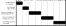
\includegraphics[width=260pt]{figuras/cronograma}
    \caption{Cronograma original do projeto}
    \label{fig-cronograma}
    \end{center}
\end{figure}

\section{Cronograma revisado}

% TODO: revisar o cronograma

==== O CRONOGRAMA FINAL SERÁ FEITO NO FIM DO PERÍODO ====

%% O plano de ação original foi levemente modificado. A validação do problema durou um pouco mais do que planejado. As etapas relacionadas ao algoritmo foram agrupadas no desenvolvimento do sistema, e foi criada uma nova etapa de elaboração de requisitos. O cronograma revisado pode ser visualizado na figura \ref{fig-cronograma-atualizado}.

\begin{figure}[ht!]
    \begin{center}
    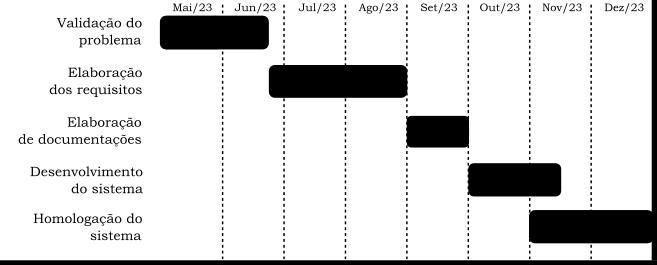
\includegraphics[width=260pt]{figuras/cronograma-atualizado}
    \caption{Cronograma atualizado do projeto}
    \label{fig-cronograma-atualizado}
    \end{center}
\end{figure}
  %% ...
  \arial
  \bibliographystyle{abnt-num} % \bibliographystyle{abnt-alf}
  \bibliography{main} 
\end{document}
